\chapter{Руководство пользователя} %todo стянуть с документации к NCC
\label{ch:usrmanual}

Разрабатываемый сервис агрегации данных по call-центру входит в состав Naumen Contact Center и поставляется вместе с ним же.
Поэтому, для общих моментов в текущем разделе будет приведено руководство пользователя по NCC\@.

\section{Установка}

%\subsection{Установка Oracle Linux 7.X} todo если будет мало текста -- раскоменнтировать и добавить недостающие пункты https://callcenter.naumen.ru/docs/ru/ncc73/ncc/web/Content/Installation/Server_OS_Installation/Linux_Oracle_Installation_Kickstart.htm

%На каждый сервер NCC должна быть установлена последняя версия ОС Oracle Linux 7.х.
%Данное описание предполагает использование сценария установки (KickStart) и описывает минимальные действия, необходимые для установки ОС Oracle Linux 7.х.
%
%Версия операционной системы Oracle Linux должна быть не ниже версии 7.2.
%
%Дистрибутив Oracle Linux доступен на сайте Oracle (https://edelivery.oracle.com/linux) после предварительной регистрации.
%
%Для установки ОС выполните следующие действия:

Naumen Contact Center устанавливается при помощи мастера установки, работа с которым осуществляется посредством Web-интерфейса.

Для установки выполните следующие действия:
\begin{enumerate}
    \item подключитесь к мастеру установки: откройте интернет-обозреватель и перейдите по адресу \texttt{https://hostname:8001}, где \texttt{hostname} — IP-адрес сервера, на который был установлен пакет \texttt{ncc-installer};
    \item подключитесь к системе Server Access: Укажите имя пользователя и пароль для доступа к личному кабинету системы Server Access;
    \item укажите параметры инсталляции, если на рабочих местах операторов используется операционная система Ubuntu Linux, установите флажок Установить NSP репозиторий;
    \item укажите параметры соединения для серверов и баз данных;
    \item мастер запустит ряд проверок. После прохождения проверок нажмите на кнопку \texttt{Далее};
    \item укажите соответствие ролей серверам. Для этого для каждого сервера отметьте (установите флажок) роли, которые он будет выполнять;
    \item если при использовании NCC планируется использовать WebPhone, установите флажок в поле Включить WebRTC;
    \item настройте параметры межсетевого экрана:
    \begin{enumerate}
        \item если настройка межсетевого экрана уже была произведена вручную после установки ОС и все настройки были выполнены в соответствии с политикой безопасности компании, установите флажок \texttt{Не производить настройку межсетевого экрана}.
        \item по умолчанию добавлены следующие подсети: 10.0.0.0/8, 172.16.0.0/12, 192.168.0.0/16
        \item при необходимости в поле Открыть доступ для укажите подсеть, клиентам которой необходим доступ к Системе. Подсеть указывается в формате: \verb|<адрес_подсети>/<длина_префикса>|;
        \item чтобы добавить дополнительные подсети воспользуйтесь ссылкой \texttt{Добавить подсеть} и укажите их адреса;
    \end{enumerate}
    \item при необходимости настройки имени сервера (hostname) убедитесь, что флажок \texttt{Изменить имена серверов} установлен и укажите имя в поле \texttt{Имя сервера} для каждого сервера;
    \item если на основном сервере несколько сетевых интерфейсов, выберите сетевой интерфейс для взаимодействия программных IP-телефонов SoftPhone с сервером по протоколу SIP;
    \item при обновлении NCC, если в предыдущей версии был указан хотя бы один параметр интеграции с Web-системой, в мастере установки будет отображаться блок \texttt{ИНТЕГРАЦИЯ С WEB-СИСТЕМОЙ};
    \item запустите процесс установки.
\end{enumerate}

В результате приведенных выше действий мастер установит NCC\@.

После успешной установки NCC в верхней части страницы появятся ссылки, которые позволяют:
\begin{itemize}
    \item перейти в систему управления проектами;
    \item получить сценарий для установки Naumen SoftPhone на рабочие места с операционной системой Ubuntu Linux.
\end{itemize}

Если процесс установки завершен успешно, остановите и удалите мастер установки с сервера, на котором он был установлен, выполнив в консоли следующие команды:
\begin{verbatim}
    # service ncc-installer stop
    # yum erase ncc-installer-ru
\end{verbatim}

\section{Требуемые ресурсы}

\subsection{Требования к конфигурации и аппаратному обеспечению серверов}
\label{subsec:system:req}

Конфигурация каждого контактного центра чаще всего уникальна и зависит от множества параметров,
таких как использование резервирования, конфигурация аппаратного обеспечения, конфигурация проектов,
бизнес-процессов, планируемой нагрузки и т.~п.

В таблице~\ref{tab:system:req} приведены минимальные требования к конфигурации
и аппаратному обеспечению серверов для контактных центров без использования резервирования
(в зависимости от количества операторских рабочих мест).

\begin{table}[!htp]
    \caption{Минимальные требования к конфигурации и аппаратному обеспечению}
    \begin{small}
        \begin{tabular}{|p{0.2\textwidth}                |p{0.2\textwidth}         |p{0.2\textwidth}                                                           |p{0.1\textwidth}              |p{0.15\textwidth}|}
        \hline
        Количество операторов         & Сервер                  & Процессор                                                              & Объем оперативной памяти (ГБ)& Объем жесткого диска \\
        \hline
        \multirow{5}{*}{от 200 до 650}& Основной сервер         & \multirow{5}{0.2\textwidth}{Intel Core i7-4770 / Intel Xeon E5-1630 v4}& \multirow{5}{*}{32}          & \multirow{5}{0.15\textwidth}{2 ТБ Enterprise sata} \\
                                      & Коммутационный сервер   &                                                                        &                              & \\
                                      & Сервер звукозаписи      &                                                                        &                              & \\
                                      & Сервер PMS              &                                                                        &                              & \\
                                      & Сервер отчетов          &                                                                        &                              & \\
        \hline
        \multirow{6}{*}{от 650 до 700}& Основной сервер         & \multirow{6}{0.2\textwidth}{Intel Core i7-4770 / Intel Xeon E5-1630 v4}& \multirow{5}{*}{32}          & \multirow{5}{0.15\textwidth}{2 ТБ Enterprise sata} \\
                                      & Коммутационный сервер   &                                                                        &                              & \\
                                      & Сервер звукозаписи      &                                                                        &                              & \\
                                      & Сервер PMS              &                                                                        &                              & \\
                                      & Сервер отчетов          &                                                                        &                              & \\
        \cline{2-2}\cline{4-5}
                                      & Коммутационный сервер x2&                                                                        & 64                           & 240 ГБ SSD \\
        \hline
        \end{tabular}
    \end{small}
    \label{tab:system:req}
\end{table}

%При организации контактного центра обратите внимание на следующие рекомендации:
%
%При выборе процессора учитывайте частоту и размер кэша.
%
%Количество ядер процессора для коммутационного сервера рассчитывается из условия, что один сервис Tel занимает одно ядро процессора и способен обслуживать до 200 одновременных соединений. Не рекомендуется размещать более 6 сервисов Tel на одном сервере.
%
%При высокой нагрузке на Сервер PMS (PMS) выделяйте Сервер отчетов (Reports) и Сервер БД в отдельный сервер.
%
%При расчете необходимого объема жестких дисков необходимо предусмотреть возможность хранения незакодированных записей разговоров в течение 2-3 суток. Объем зависит от числа одновременно записываемых звуковых потоков. Одна минута незакодированных звуковых данных занимает ~2 МБ на жестком диске. Поэтому один поток незакодированных звуковых данных будет заполнять диск со скоростью 120 Мб в час (или 2,9 Гб в сутки). Для записи одного телефонного разговора обычно используется 2 потока.
%
%Для повышения скорости записи диски рекомендуется объединять в RAID-массив 0, 6 или 10 уровня. Все сервисы Tel, при включенной записи разговоров, активно записывают звуковые данные на жесткий диск. Поэтому нужно правильно рассчитывать максимально возможное количество одновременных вызовов на каждом сервере, исходя из возможностей дисковой подсистемы. Необходимо исходить из расчета, что одну запись разговора необходимо записывать со скоростью ~4 Мб в минуту.
%
%Количество ядер процессора для сервера звукозаписи рассчитывается из условия, что один сервис RecConv занимает одно ядро процессора. Один сервис RecConv способен конвертировать записи разговора примерно 100 работающих операторов. Если записывать все, в том числе и во время нахождения вызова на IVR, то необходимо исходить из расчета 2 сервиса RecConv на 1 сервис Tel.
%
%Необходимый объем жесткого диска для хранения записей зависит от количества одновременно записываемых звуковых потоков, формата записи и хранения телефонных переговоров и требуемого времени хранения записей разговоров. Скорость наполнения жесткого диска (в Мб/час) при записи нескольких потоков рассчитывается по формуле:
%
%Для формата моно — Vчас = 6Мб/час*N.
%
%Для формата стерео — Vчас = 9Мб/час*N.
%
%Где N — число одновременно записываемых звуковых потоков.
%
%Чтобы рассчитать время (в часах), в течение которого заполнится объем жесткого диска, необходимо использовать формулу:
%
%T = Wдиск/Vчас,
%
%где Wдиск — объем жесткого диска в МБ, Vчас — скорость наполнения жесткого диска в Мб/час.
%
%Для повышения надежности диски рекомендуется объединять в RAID-массив 0, 6 или 10 уровня.
%
%В Системе обычно используются СУБД Oracle или PostgreSQL, в которых хранится как статистическая информация, так и системные данные.

\subsection{Требования к серверному программному обеспечению}

\subsubsection{Требования к серверной операционной системе}

Требования к операционным системам для описанных в разделе \S~\ref{subsec:system:req} типов серверов представлены ниже.

На каждом сервере должна быть установлена последняя версия операционной системы Oracle Linux 7.х (бесплатная).
Установка ОС Oracle Linux рассмотрена в разделе «Установка ОС Oracle Linux 7.х». %todo сделать ссылку, после того как будет заполнен раздел

Рекомендуется устанавливать 64-разрядную версию ОС.
В случае, если на сервере используется более 4 Гб оперативной памяти, ОС обязательно должна быть 64-разрядной.

Версия операционной системы Oracle Linux должна быть не ниже версии 7.2.

Возможна совместимость с ОС RedHat Enterprise Linux (платная), CentOS (бесплатная).
За дополнительной информацией обратитесь к специалистам компании Naumen.

\subsubsection{Требования к СУБД}

На каждом сервере БД должна быть установлена одна из следующих СУБД:
\begin{itemize}
    \item PostgreSQL 9.6;
    \item Oracle Database 11g Release 2. %todo ссылка на установку
\end{itemize}

Должна быть создана учетная запись пользователя, от имени которой Система будет работать с БД.
Данной учетной записи пользователя должны быть назначены права на подключение и создание основных объектов в БД, см следующие разделы: %todo добавить следующие разделы

%
%Установка Oracle 11g
%
%Создание базы данных Oracle 11g
%
%Настройка Oracle 11g
%
%
%«Установка PostgreSQL 9.6» (шаг 5).
%
%«Настройка Oracle 11g» (шаг 7).


\subsection{Требования к ЛВС}

\Abbrev{LAN}{ЛВС --- локальная вычислительная сеть}
\Abbrev{VoIP}{Voice-over-IP --- телефонная связь по протоколу IP}
\Define{Full duplex}{дуплексная радиосвязь предусматривает одновременную двустороннюю передачу информации}
При построении локальной вычислительной сети (LAN) следует придерживаться следующих требований:
\begin{enumerate}
    \item сеть для передачи VoIP трафика должна строиться на основе коммутаторов работающих в режиме полного дуплекса (full duplex);
    \item общая задержка между начальной и конечной точкой приема и передачи голосовых данных не должна превышать 150--200мс;
    \item потери пакетов в сети по пути следования голосового трафика не должны превышать 3\%;
    \item пропускная способность каналов передачи данных должна быть достаточной для одновременного прохождения необходимого количества голосовых потоков закодированных определенным кодеком:
    \begin{enumerate}
        \item для одного канала при использовании кодека G.711 необходимая пропускная способность должна быть не менее ~80 Кбит/c в одну сторону;
        \item для одного канала необходимая пропускная способность при использовании кодека G.729 должна быть не менее ~20 Кбит/c в одну сторону;
    \end{enumerate}
    \item между пользователями контактного центра и серверами NCC, а также устройствами интеграции с другими сетями (VoIP-шлюзы, УАТС и т.~д.) и серверами NCC не должно быть устройств, осуществляющих трансляцию IP-адресов (NAT) или фильтрацию IP-пакетов (межсетевой экран), препятствующих прохождению VoIP-трафика. Для обхода NAT чаще всего используется технология VPN, либо STUN-серверы. Допускается использовать NAT в следующих случаях:
    \begin{enumerate}
        \item оператор использует WebPhone. При этом NAT должен быть не симметричным и межсетевые экраны на всех промежуточных шлюзах не должны блокировать входящий трафик;
        \item оператор использует SoftPhone. При этом протокол ICE должен быть включен и настроен в конфигурационном файле сервиса Tel, в параметрах профиля пользователя должны быть настроены параметры сервера STUN;
    \end{enumerate}
    \item при построении сети с применением средств VPN и при использовании для передачи голоса открытых сетей (Интернет), требования остаются аналогичными описанным выше;
    \item между пользователями контактного центра и серверами NCC, между серверами NCC, а также между серверами NCC и другими системами, осуществляющими взаимодействие с серверами NCC, не должны блокироваться необходимые для работы порты и протоколы;
    \item при построении высоко нагруженных систем с числом операторов 500 и выше серверы NCC должны объединяться в сеть, построенную с использованием технологии Gigabit Ethernet;
\end{enumerate}

\section{Порядок работы}

\subsection{Общая информация об отчетах реального времени}

В NCC присутствуют отчеты реального времени по проектам типа Очередь (входящий) и Обзвон (исходящий), при этом возможны следующие варианты:
\begin{itemize}
    \item если отчет относится к типу проекта Очередь, то это означает, что информация в отчете может быть отражена
    только по проектам данного типа;
    \item если отчет относится к типу проекта Обзвон,
    то это означает, что информация в отчете может быть отражена только по проектам данного типа;
    \item если отчет относится к обоим типам проектов, то это означает, что информация в отчете объединяет информацию по обоим типам проектов.
\end{itemize}

Процесс выбора проектов для отображения рассмотрен в разделе~\S~\ref{subsec:выбор-проектов-для-отображения}.

Отчеты, по способу представления, можно разделить на три типа:
\begin{enumerate}[1)]
    \item сводки --- информация отображается в виде карточек, содержащих показатели и графики;
    \item таблицы --- информация отображается в виде таблицы;
    \item графики --- информация отображается в виде графиков.
\end{enumerate}

Доступные на данный момент в NCC отчеты реального времени представлены в таблице~\ref{tab:orders}.

\begin{table}[ht]
    \caption{Отчеты реального времени}
    \begin{small}
        \begin{tabular}{|p{0.35\textwidth}|p{0.15\textwidth}|p{0.2\textwidth}|p{0.15\textwidth}|}
            \hline
            Отчет & Тип проекта & Уровень & Тип отчета \\
            \hline
            Сводки по входящим проектам & Очередь & Компания, Партнер & Сводка  \\
            \hline
            Отчет по входящим проектам & Очередь & Компания, Партнер & Таблица  \\
            \hline
            Отчет по операторам & Очередь, Обзвон & Компания, Отдел (сотрудники отдела, включая подотделы), Проект (участники проекта) & Таблица  \\
            \hline
            График изменения ключевых показателей & Очередь & Проект & График  \\
            \hline
        \end{tabular}
    \end{small}
    \label{tab:orders}
\end{table}

Отчеты реального времени доступны для просмотра на различных уровнях иерархии объектов PMS, что обеспечивает следующие важные возможности и особенности:
\begin{itemize}
    \item на каждом уровне могут быть настроены различные права на просмотр;
    \item в зависимости от того, на каком уровне открыт отчет по проектам или операторам, будет доступен для отображения различный перечень проектов или различный состав участников проекта соответственно;
    \item в зависимости от того, на каком уровне открыт отчет, будет доступен для отображения различный перечень показателей;
    \item отчет можно найти на указанном в таблице выше уровне, а именно в блоке <<ОТЧЕТЫ РЕАЛЬНОГО ВРЕМЕНИ>> вкладки <<Отчеты>> карточки объекта (рисунок~\ref{pic:realtimereports}).
\end{itemize}

\begin{figure}[ht]
    
\includegraphics[width=0.85\textwidth]{inc/img/realtime_reports}
    \caption{Отчеты реального времени}
    \label{pic:realtimereports}
\end{figure}

\subsection{Сводки по входящим проектам}

Отчет <<Сводки по входящим проектам>> содержит сводную информацию по выбранным проектам (рисунок~\ref{pic:intr:proj:incoming:total}).

Заголовок сводки, содержащий название проекта, является ссылкой, с помощью которой можно перейти на карточку проекта.
Под заголовком сводки может отображаться дополнительная строка, отображающая текущий режим обслуживания.
Строка отображается только в случае, если текущий режим отличается от режима <<Обычный>>.

При наведении указателя мыши на правый верхний угол сводки появляются две кнопки, см.~рисунок~\ref{pic:intr:proj:incoming:total:setting}.

\begin{figure}[ht]
    \centering
%     [width=0.5\textwidth] --- регулировка ширины картинки
    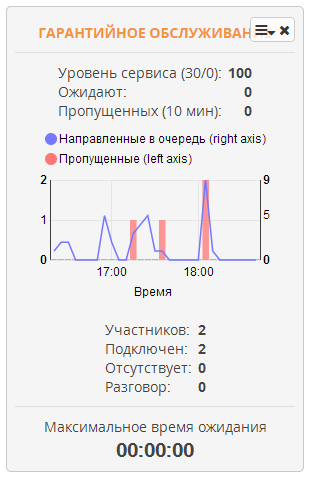
\includegraphics[width=0.6\textwidth]{inc/img/intr_incoming_ttl_setting}
    \caption{Кнопка настройки сводки по входящим проектам}
    \label{pic:intr:proj:incoming:total:setting}
\end{figure}

При нажатии на кнопку удаления сводка по отображаемому проекту будет закрыта.

При нажатии на кнопку <<Открыть меню>> открывается меню, позволяющее осуществлять оперативные действия по управлению проектом (см.~раздел~\S~\ref{subsec:оперативные-действия}).
Помимо оперативных действий в меню присутствуют два дополнительных пункта, рассмотренных в таблице~\ref{tab:prj:incoming:ttl:setting}.

\begin{table}[ht]
    \caption{Настройка сводки по входящему проекту}
    \begin{small}
        \begin{tabular}{|p{0.15\textwidth}|p{0.8\textwidth}|}
            \hline
            Действие & Описание \\
            \hline
            Параметры отображения & При выборе данного пункта меню открывается форма <<НАСТРОЙКА ОТОБРАЖЕНИЯ ОТЧЕТОВ РЕАЛЬНОГО ВРЕМЕНИ>> (см.~раздел~\ref{subsec:настройка-отчетов-реального-времени}).\\
            \hline
            Открыть график & При выборе данного пункта меню открывается отчет реального времени <<График изменения ключевых показателей>> по соответствующему проекту (см.~раздел~\ref{subsec:график-изменения-ключевых-показателей}).\\
            \hline
        \end{tabular}
    \end{small}
    \label{tab:prj:incoming:ttl:setting}
\end{table}

Графики отображаются за последние 4 часа с шагом в 5 минут.
Описание графиков, расположенных на сводке, рассмотрено в таблице~\ref{tab:prj:incoming:ttl:charts}.

\begin{table}[ht]
    \caption{Настройка сводки по входящему проекту}
    \begin{small}
        \begin{tabular}{|p{0.15\textwidth}|p{0.8\textwidth}|}
            \hline
            График & Описание \\
            \hline
            Направленные в очередь (right axis) & График отражает количество вызовов, распределившихся из очереди и уже успешно обработанных оператором (т.~е. уже завершенных вызовов). График отображается в виде синей ломанной линии, данному графику соответствует шкала справа.\\
            \hline
            Пропущенные (left axis) & График отражает количество пропущенных вызовов, (т. е. вызовов, завершившихся во время ожидания ответа оператора в очереди и не распределившихся на оператора). При этом не учитываются короткие пропущенные вызовы и вызовы, которые не были разблокированы. График отображается в виде красных столбиков, для данного графика соответствует шкала слева.\\
            \hline
        \end{tabular}
    \end{small}
    \label{tab:prj:incoming:ttl:charts}
\end{table}

Описание приведенных на сводке показателей представлено в таблице~\ref{tab:prj:incoming:ttl:indicators},
для получение более подробной информации см.~раздел~\S~\ref{subsec:показатели-эффективности}.
Отображение некоторых из показателей можно настраивать, подробнее об этом в разделе~\S~\ref{subsec:настройка-отчетов-реального-времени}

\Abbrev{SL}{Service Level --- уровень сервиса}
\begin{table}[ht]
    \caption{Описание показателей сводки по входящим проектам}
    \begin{small}
        \begin{tabular}{|p{0.15\textwidth}|p{0.7\textwidth}|p{0.1\textwidth}|}
            \hline
            Показатель & Описание & Формат \\
            \hline
            Уровень сервиса & Соответствует показателю для входящего проекта <<Уровень сервиса>> (SL).
            Показатель может подсвечиваться. & -- \\
            \hline
            Ожидают &
            Соответствует показателю для входящего проекта <<Вызовы в очереди>> (Calls in Queue).
            Показатель может подсвечиваться. & --\\
            \hline
            Пропущенных &
            Соответствует показателю для входящего проекта <<Потерянные вызовы>> (Abandoned Calls).
            Показатель может подсвечиваться. & -- \\
            \hline
            Участников &
            Общее количество операторов, назначенных на проект. &
            Целое число. \\
            \hline
            Подключен &
            Количество операторов, зарегистрированных в системе в данный момент (онлайн). &
            Целое число. \\
            \hline
            Отсутствует &
            Количество операторов, находящихся в состоянии <<Отсутствует>> и <<Не беспокоить>>. &
            Целое число. \\
            \hline
            Разговор &
            Количество операторов, находящихся в состоянии <<Разговор>>. &
            Целое число. \\
            \hline
            Максимальное время ожидания &
            Соответствует показателю для входящего проекта Максимальное время ожидания (Longest Call Waiting). &
            -- \\
            \hline
        \end{tabular}
    \end{small}
    \label{tab:prj:incoming:ttl:indicators}
\end{table}

\subsection{Отчет по входящим проектам}

Отчет по входящим проектам содержит информацию по выбранным проектам (рисунок~\ref{pic:intr:proj:incoming}).

В зависимости от настройки отображения полей, таблица может содержать следующие поля:
\begin{itemize}
    \item поле <<Проект>> --- название проекта, является ссылкой на карточку проекта;
    \item поле <<Состояние проекта>> --- текущее состояние проекта: <<Активный>> или <<Блокированный>>;
    \item поля, соответствующие показателям, рассмотренным в разделе «Показатели эффективности для входящих проектов».
\end{itemize}

При нажатии на кнопку <<Открыть меню>> открывается меню, позволяющее осуществлять оперативные действия по управлению проектом
(см.~раздел~\S~\ref{subsec:оперативные-действия}).
Помимо оперативных действий в меню присутствует дополнительный пункт <<Редактировать условия подсветки>>.
При выборе данного пункта открывается форма <<РЕДАКТИРОВАНИЕ УСЛОВИЙ ПОДСВЕТКИ>>,
позволяющая настраивать условия подсветки для значений показателей в таблице.
Для получения более подробной информации по работе с данной формой,
а также другом способе ее открытия см.~раздел~\S~\ref{subsec:настройка-отчетов-реального-времени}.

В данном отчете присутствует возможность сохранения данных локально в файле формата Excel.
Для этого необходимо в блоке, название которого соответствует названию отчета,
нажать на кнопку <<Выгрузить в Excel>>.
После нажатия кнопки файл будет сохранен в каталог по умолчанию для сохранения загружаемых файлов
и может быть открыт в MS Excel для редактирования.

\subsection{Отчет по исходящим проектам}

Отчет по исходящим проектам содержит информацию по выбранным проектам (рисунок~\ref{pic:intr:proj:outcoming}).

В зависимости от настроек отображения (см.~раздел~\S~\ref{subsec:настройка-отчетов-реального-времени}), таблица может содержать два типа полей:
\begin{itemize}
    \item поля, содержащие информацию о проекте. Описание полей приведено в таблице~\ref{tab:prj:incoming:fields};
    \item поля, содержащие показатели эффективности (см.~раздел~\S~\ref{subsec:показатели-эффективности}).
\end{itemize}
\begin{table}[ht]
    \caption{Поля в отчете по входящим проектам}
    \begin{small}
        \begin{tabular}{|p{0.15\textwidth}|p{0.8\textwidth}|}
            \hline
            Поле & Описание \\
            \hline
            Проект & Состояние проекта: <<Активный>> или <<Блокированный>>. \\
            \hline
            Состояние проекта & Название проекта, является ссылкой на карточку проекта. \\
            \hline
            Состояние обзвона & Может быть:
            \begin{itemize} %todo настроить отсутпы нумерации в таблице
                \item <<Обзвон не выгружен>>,
                \item <<Активный>>,
                \item <<Приостановлен>>,
                \item <<Завершен>>,
                \item <<Неизвестно>>,
                \item <<Ошибка>>.
            \end{itemize}
            Пустое поле --- полуавтоматический тип обзвона. \\
            \hline
            Режим обзвона & Режим автоматического исходящего обзвона. Возможные значения:
            \begin{itemize}
                \item <<Предиктивный>>,
                \item <<Предиктивный (упрощенный)>>,
                \item <<Прогрессивный>>,
                \item <<Прогрессивный через QPM>>,
                \item Полуавтоматический.
            \end{itemize} \\
            \hline
            Открыть меню & Поле содержит кнопку <<Открыть меню>>.
            Кнопка открывает меню, позволяющее осуществлять оперативные действия по управлению проектом
            (см.~раздел~\S~\ref{subsec:оперативные-действия}).
            Помимо оперативных действий в меню присутствует дополнительный пункт <<Редактировать условия подсветки>>.
            При выборе данного пункта открывается форма <<РЕДАКТИРОВАНИЕ УСЛОВИЙ ПОДСВЕТКИ>>,
            позволяющая настраивать условия подсветки для значений показателей в таблице.
            Для получения более подробной информации по работе с данной формой,
            а также другом способе ее открытия см.~раздел~\S~\ref{subsec:настройка-отчетов-реального-времени}. \\
            \hline
        \end{tabular}
    \end{small}
    \label{tab:prj:incoming:fields}
\end{table}

В данном отчете присутствует возможность сохранения данных локально в файле формата Excel.
Для этого необходимо в блоке, название которого соответствует названию отчета, нажать на кнопку <<Выгрузить в Excel>>.
После нажатия кнопки файл будет сохранен в каталог по умолчанию для сохранения загружаемых файлов и может быть открыт в MS Excel для редактирования.

\subsection{Отчет по операторам}

Отчет <<Отчет по операторам>>, в зависимости от уровня иерархии на котором он открыт,
содержит информацию по операторам проекта, отдела или всей компании (рисунок~\ref{pic:intr:operator}).

Таблица может содержать поле Оператор, содержащее имя оператора, а также показатели, рассмотренные в разделе~\S~\ref{subsec:показатели-эффективности}.
<<Имя оператора>> является ссылкой, с помощью которой можно перейти на карточку оператора.

В данном отчете присутствует возможность сохранения данных локально в файле формата Excel.
Для этого необходимо в блоке, название которого соответствует названию отчета, нажать на кнопку <<Выгрузить в Excel>>.
После нажатия кнопки файл будет сохранен в каталог по умолчанию для сохранения загружаемых файлов и может быть открыт в MS Excel для редактирования.

\subsection{График изменения ключевых показателей}\label{subsec:график-изменения-ключевых-показателей}

Отчет <<График изменения ключевых показателей>> содержит графики изменения ключевых показателей во времени.
Основное назначение графиков --- быстро отследить зависимости между изменениями значений ключевых показателей.
Например, из графиков можно легко увидеть чем обусловлено падение уровня сервиса.
Иногда причиной может быть увеличение количества поступивших в очередь вызовов,
но на рисунке~\ref{pic:intr:proj:keyval} можно легко заметить, что причиной было увеличение времени обработки вызовов.

Графики можно отобразить для следующих показателей:
\begin{itemize}
    \item уровень сервиса;
    \item направленные в очередь вызовы;
    \item среднее время обработки вызова (в секундах);
    \item среднее время ожидания (в секундах);
    \item среднее время разговора (в секундах);
    \item среднее время поствызывной обработки (в секундах).
\end{itemize}

Описание приведенных выше показателей можно найти в разделе~\S~\ref{subsec:показатели-эффективности}.

При наведении указателя мыши на область построения графиков отображается всплывающее информационное окно содержащее значения показателей
в указанное время, время и значения показателей соответствуют положению указателя относительно временной шкалы.
При наведении указателя на какой-либо график, во всплывающем окне выделяется показатель, соответствующий графику.

Отчет предусматривает возможность отображения и скрытия тех или иных графиков.
В верхней части отчета перечислены все возможные для отображения графики.
При нажатии на тот или иной показатель, соответствующий график отображается или скрывается.
Отображен график или скрыт можно понять по значку в виде кругляшка слева от показателя.
Если кругляшок закрашен, то график отображается, если не закрашен, то график не отображается.

Графики отображаются максимум за последние 8 часов с минимальным шагом в 5 минут.

В данном отчете присутствует возможность выполнять оперативные действия.
Оперативные действия доступны в выпадающем списке <<Управление проектом>> в левом верхнем углу блока <<ГРАФИК ИЗМЕНЕНИЯ КЛЮЧЕВЫХ ПОКАЗАТЕЛЕЙ>>.
Описание доступных действий приведено в разделе~\S~\ref{subsec:оперативные-действия}.

\subsection{Оперативные действия}\label{subsec:оперативные-действия}

В отчетах реального времени предусмотрена возможность осуществления оперативных действий по управлению проектами.
В каждом отчете реального времени набор возможных действий отличается.

В таблице~\ref{tab:actions} рассмотрены возможные оперативные действия с указанием отчетов, в которых они доступны.


\begin{small}
\begin{longtable}{|p{0.2\textwidth}|p{0.25\textwidth}|p{0.5\textwidth}|}
    \caption{Оперативные действия}
    \label{tab:actions}
    \\ \hline
    Действие & Отчет & Описание \\
    \hline \endfirsthead
    \hline
    Действие & Отчет & Описание \\
    \hline
    \endhead
    \hline \endlastfoot
    Изменить набор операторов &
    Сводки по входящим проектам &
    При выборе данного пункта меню открывается форма
    <<ИЗМЕНЕНИЕ НАБОРА ОПЕРАТОРОВ>>. \\
    \hline
    Отправить сообщение операторам &
    График изменения ключевых показателей;
    Сводки по входящим проектам;
    Отчет по входящим проектам;
    Отчет по исходящим проектам. &
    При выборе данного пункта можно отправить текстовое сообщение
    всем операторам проекта. \\
    \hline
    Изменить приоритет очереди &
    График изменения ключевых показателей;
    Сводки по входящим проектам;
    Отчет по входящим проектам. &
    При выборе данного пункта меню открывается форма
    <<ИЗМЕНЕНИЕ ПРИОРИТЕТА ОЧЕРЕДИ>> на которой можно
    указать необходимый приоритет для вызовов очереди проекта.\\
    \hline
    Изменить режим обслуживания &
    График изменения ключевых показателей;
    Сводки по входящим проектам;
    Отчет по входящим проектам. &
    При выборе данного пункта меню открывается форма
    <<ИЗМЕНЕНИЕ РЕЖИМА ОБСЛУЖИВАНИЯ ОЧЕРЕДИ>> на которой можно выбрать
    необходимый режим обслуживания очереди обработки вызовов.\\
    \hline
    Изменить количество попыток дозвона на номер &
    Отчет по исходящим проектам. &
    При выборе данного пункта меню открывается форма
    <<ИЗМЕНЕНИЕ КОЛИЧЕСТВА ПОПЫТОК ДОЗВОНА НА НОМЕР>>
    на которой можно указать количество попыток дозвона
    на номер во время телефонного обзвона.\\
    \hline
    Изменить режим обзвона &
    Отчет по исходящим проектам. &
    При выборе данного пункта меню открывается форма
    <<ИЗМЕНЕНИЕ РЕЖИМА ОБЗВОНА>> на которой можно указать режим обзвона.
    Отображается только для автоматического типа обзвона. \\
    \hline
    Приостановить обзвон &
    Отчет по исходящим проектам. &
    Приостановка обзвона.
    Отображается только для рабочего состояния
    автоматического обзвона (состояние <<Активный>>).\\
    \hline
    Начать обзвон &
    Отчет по исходящим проектам. &
    Запуск или возобновление обзвона.
    Отображается только для остановленного состояния
    автоматического обзвона (состояние <<Обзвон не выгружен>> или
    <<Приостановлен>>).\\
    \hline
    Обновить список номеров &
    Отчет по исходящим проектам. &
    Обновление списка номеров.
    Отображается только для автоматического обзвона
    если кейсы выгружены (обзвон в состоянии <<Активный>> или <<Приостановлен>>).\\
\end{longtable}
\end{small}


\subsection{Выбор проектов для отображения}
\label{subsec:выбор-проектов-для-отображения}

В отчетах по проектам есть возможность выбрать проекты, информация по которым будет отображаться в отчете.

Чтобы выбрать проекты для отображения, выполните следующие действия:
\begin{enumerate}
    \item на карточке отчета нажмите на кнопку <<Выбрать проекты>>. Откроется форма <<ВЫБОР ПРОЕКТОВ>> (рисунок~\ref{pic:changeprj});
    \item в открывшейся форме установите/снимите флажки (по умолчанию установлены):
    \begin{enumerate}
        \item <<Отображать все>> --- отображать в отчете информацию по всем проектам партнера/компании;
        \item <<Скрыть блокированные>> --- не отображать в отчете информацию по проектам в состоянии <<Блокированный>>;
    \end{enumerate}
    \item если флажок <<Отображать все>> не установлен, ниже отображается список доступных проектов (рисунок~\ref{pic:intr:proj:select}). Список сгруппирован по партнерам, если отчет настраивается на уровне компании.
    \item выберите в списке проекты, которые требуется включить в отчет. Для этого:
    \begin{enumerate}
        \item если отчет настраивается на уровне компании, выделите блок с названием партнера. Ниже отобразятся проекты партнера;
        \item переместите необходимые проекты в правую область формы;
        \item повторите действия для каждого проекта, который необходимо отобразить;
        \item установите очередность расположения проектов в отчете путем перетаскиания их в правой части формы;
    \end{enumerate}
    \item нажмите на кнопку <<Сохранить>>.
\end{enumerate}

\begin{figure}[ht]
    \centering
    %     [width=0.5\textwidth] --- регулировка ширины картинки
    
\includegraphics[width=0.6\textwidth]{inc/img/intr_changeprj}
    \caption{Форма выбора проектов}
    \label{pic:changeprj}
\end{figure}

\subsection{Настройка отчетов реального времени}\label{subsec:настройка-отчетов-реального-времени}

В данном разделе рассмотрен блок <<НАСТРОЙКИ ОТЧЕТОВ РЕАЛЬНОГО ВРЕМЕНИ>>.

В блоке настраиваются параметры отчетов реального времени.

Блок отображается только в голосовых проектах с использованием очередей вызовов.

Во входящем проекте блок выглядит так, как представлено на рисунке~\ref{pic:incoming:setting}.

\begin{figure}[ht]
    \centering
    %     [width=0.5\textwidth] --- регулировка ширины картинки
    
\includegraphics[width=0.6\textwidth]{inc/img/intr_report_setting}
    \caption{Блок настройки отчетов реального времени в входящем проекте}
    \label{pic:incoming:setting}
\end{figure}

Для исходящих проектов нет отчетов типа сводка, поэтому в исходящем проекте параметры,
касающиеся сводок, отсутствуют и блок выглядит так, как представлено на рисунке~\ref{pic:outcoming:setting}.

\begin{figure}[ht]
    \centering
    %     [width=0.5\textwidth] --- регулировка ширины картинки
    
\includegraphics[width=0.6\textwidth]{inc/img/intr_outcoming_setting}
    \caption{Блок настройки отчетов реального времени в исходящем проекте}
    \label{pic:outcoming:setting}
\end{figure}

Блок позволяет выполнить следующие действия:
\begin{itemize}
    \item настроить отображение отчетов реального времени;
    \item изменить условия подсветки;
    \item настроить права на просмотр отчетов реального времени.
\end{itemize}

\subsubsection{Настройка отображения отчетов реального времени}

Чтобы настроить отображение отчетов реального времени:
\begin{enumerate}
    \item нажмите на кнопку <<Настроить отображение отчетов реального времени>>;
    \item в открывшейся форме <<НАСТРОЙКА ОТОБРАЖЕНИЯ ОТЧЕТОВ РЕАЛЬНОГО ВРЕМЕНИ>>
    измените необходимые поля (рисунок~\ref{pic:prj:setting:fields});
    \item нажмите на кнопку <<Сохранить>>.
\end{enumerate}

\begin{figure}[ht]
    \centering
    %     [width=0.5\textwidth] --- регулировка ширины картинки
    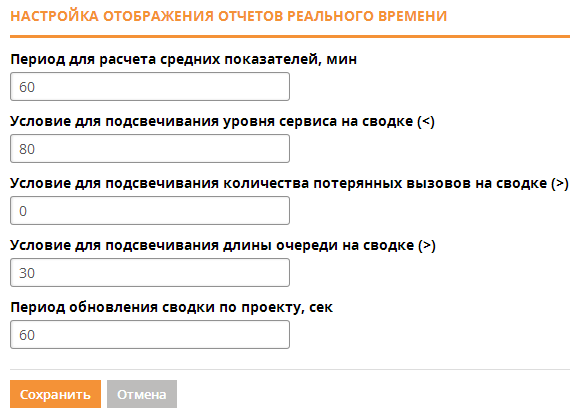
\includegraphics[width=0.6\textwidth]{inc/img/intr_prj_setting}
    \caption{Блок настройки отчетов реального времени в исходящем проекте}
    \label{pic:prj:setting:fields}
\end{figure}

Описание полей формы <<НАСТРОЙКА ОТОБРАЖЕНИЯ ОТЧЕТОВ РЕАЛЬНОГО ВРЕМЕНИ>> представлены в таблице~\ref{tab:prj:setting:fields}.
\begin{table}[ht]
    \caption{Поля в настройках отображения отчетов реального времени}
    \begin{small}
        \begin{tabular}{|p{0.2\textwidth}|p{0.4\textwidth}|p{0.15\textwidth}|p{0.1\textwidth}|}
            \hline
            Параметр & Описание & Представление отчета & Значение по умолчанию \\
            \hline
            Период для расчета средних показателей, мин &
            Интервал времени, необходимый для расчета показателей, вычисляемых за период. &
            Таблица; Сводки &
            60\\
            \hline
            Условие для подсвечивания уровня сервиса на сводке (<) &
            Условие подсвечивания для значения показателя Уровень сервиса. &
            Сводки &
            80 \\
            \hline
            Условие для подсвечивания количества потерянных вызовов (>) &
            Условие подсвечивания значения показателя Пропущенных. &
            Сводки &
            0 \\
            \hline
            Условие для подсвечивания длины очереди на сводке (>) &
            Условие подсвечивания значения показателя Ожидают. &
            Сводки &
            30 \\
            \hline
            Период обновления сводки по проекту, сек &
            Период обновления информации в сводке. &
            Сводки &
            60 \\
            \hline
        \end{tabular}
    \end{small}
    \label{tab:prj:setting:fields}
\end{table}

\subsubsection{Редактирование условий подсветки}

Условия подсветки определяют диапазоны, при выходе за пределы которых значения
в отчетах табличного вида по входящим и исходящим проектам будут
подсвечиваться красным цветом.
Минимальное значение диапазона определяется полем <<Мин. значение>>,
максимальное значение диапазона определяется полем <<Макс. значение>>.

Минимальное значение не должно превышать максимальное.

Чтобы изменить условия подсветки:
\begin{enumerate}
    \item Нажмите на кнопку <<Редактировать условия подсветки>>.
    \item В открывшейся форме <<РЕДАКТИРОВАНИЕ УСЛОВИЙ ПОДСВЕТКИ>> измените необходимые поля.
    \item Нажмите на кнопку <<Сохранить>>.
\end{enumerate}

Поля формы <<РЕДАКТИРОВАНИЕ УСЛОВИЙ ПОДСВЕТКИ>> соответствуют показателям эффективности
для входящих и исходящих проектов. Описание показателей можно найти в разделе~\S~\ref{subsec:показатели-эффективности}.

\subsection{Показатели эффективности}\label{subsec:показатели-эффективности}

Показатели эффективности для входящих проектов и их описание представлены в таблице~\ref{tab:effectivevalue}.

\begin{small}
    \begin{longtable}{|p{0.15\textwidth}|p{0.5\textwidth}|p{0.1\textwidth}|p{0.15\textwidth}|}
        \caption{Показатели эффективности}
        \label{tab:effectivevalue}
        \\ \hline
        Наименование элемента & Содержание & Формат & Период \\
        \hline \endfirsthead
        \hline
        Наименование элемента & Содержание & Формат & Период \\
        \hline
        \endhead
        \hline \endlastfoot
        Поступившие вызовы (с начала суток) &
        Общее количество поступивших вызовов. &
        Целое число. &
        С начала суток. \\
        \hline
        Направленные в очередь вызовы &
        Общее количество вызовов, попавших в очередь. Учитываются только разблокированные вызовы. &
        Целое число. &
        Период, определенный параметром. \\
        \hline
        Вызовы в очереди &
        Количество вызовов в очереди. Учитываются только разблокированные вызовы. &
        Целое число. &
        Текущий момент времени. \\
        \hline
        Среднее время ожидания (ASA) &
        Среднее время ожидания ответа оператора, или, другими словами, среднее время нахождения вызова в очереди.
        Учитываются только разблокированные и принятые оператором вызовы. &
        Время в формате hh:mm:ss. &
        Период, определенный параметром. \\
        \hline
        Уровень сервиса (SL) &
        Доля своевременно принятых вызовов от общего числа поступивших в очередь вызовов. &
        Процент до сотых долей. &
        Период, определенный параметром. \\
        \hline
        Cвоевременно отвеченные вызовы &
        Количество вызовов, принятых в течение заданного пороговым значением времени. &
        Целое число. &
        Период, определенный параметром. \\
        \hline
        Доля потерянных вызовов &
        Доля потерянных вызовов без учета коротких потерянных вызовов,
        см. описание параметра <<Неактуальные пропущенные вызовы>>. &
        Процент до сотых долей. &
        Период, определенный параметром. \\
        \hline
        Потерянные вызовы &
        Общее количество потерянных вызовов без учета коротких.
        Учитываются только разблокированные вызовы. &
        Целое число. &
        Период, определенный параметром. \\
        \hline
        Неактуальные пропущенные вызовы &
        Количество коротких потерянных вызовов. &
        Целое число. &
        Период, определенный параметром. \\
        \hline
        Среднее время ожидания до потери вызова &
        Среднее время нахождения в очереди потерянных вызовов (показатель толерантности клиентов). &
        Время в формате hh:mm:ss. &
        Период, определенный параметром. \\
        \hline
        Среднее время реакции на звонок &
        Среднее время поднятия трубки оператором, т. е. время между распределением вызова на оператора и временем ответа оператора. &
        Время в формате hh:mm:ss. &
        Период, определенный параметром. \\
        \hline
        Среднее время разговора &
        Среднее время разговора абонента с оператором.
        Учитывается время разговора только первого оператора, время обработки вызова при его перенаправлении на других сотрудников не учитывается. &
        Время в формате hh:mm:ss. &
        Период, определенный параметром. \\
        \hline
        Среднее время поствызывной обработки &
        Среднее время поствызывной обработки вызова.
        Время считается только после завершения поствызывной обработки
        (например, когда оператор перешел в состояние <<Нормальное>>). &
        Время в формате hh:mm:ss. &
        Период, определенный параметром. \\
        \hline
        Вызовы в поствызывной обработке &
        Количество вызовов, находящихся в поствызывной обработке в данный момент времени. &
        Целое число. &
        Текущий момент времени. \\
        \hline
        Расчетное время ожидания &
        Текущее расчетное время ожидания. &
        Время в формате hh:mm:ss. &
        Текущий момент времени. \\
        \hline
        Операторы в работе &
        Количество операторов, занятых обслуживанием вызова (в состоянии <<Разговор>>),
        получивших, но еще не принявших вызов или занятых набором номера
        (в состоянии <<Звонок>>),
        а также операторов, занятых поствызывной обработкой
        (в состоянии <<Поствызывная обработка>>). &
        Целое число. &
        Текущий момент времени. \\
        \hline
        Свободные операторы &
        Количество операторов,
        готовых принять вызов в данный момент (т.~е. в состоянии <<Нормальное>>). &
        Целое число. &
        Текущий момент времени. \\
        \hline
        Доля свободных операторов &
        Доля свободных операторов от общего количества операторов. &
        Процент до сотых долей. &
        Текущий момент времени.\\
        \hline
        Отсутствующие операторы &
        Количество операторов, не готовых принять вызов (например, в состоянии <<Отсутствует>>, <<Не беспокоить>> и т.~д.). &
        Целое число. &
        Текущий момент времени.\\
        \hline
        Вызовы в обработке &
        Количество вызовов, обслуживаемых операторами в данный момент времени. &
        Целое число. &
        Текущий момент времени. \\
        \hline
        Среднее время обработки вызова (AHT) &
        Среднее время обработки вызова &
        Время в формате hh:mm:ss. &
        Период, определенный параметром.\\
        \hline
        Режим обслуживания &
        Текущий режим работы очереди обработки вызовов проекта.
        Режим выбирается при настройке параметров очереди обращений. &
        Строка. &
        Текущий момент времени. \\
        \hline
        Ожидающие обратные вызовы &
        Число абонентов, ожидающих обратного вызова. &
        Целое число. &
        Текущий момент времени. \\
    \end{longtable}
\end{small}

\section{Регламентные работы}

С каждым клиентом отдельно может заключаться договор о технической поддержки, оказываемой со сторны Naumen.

Раз в пол года сотрудниками компании Naumen или ее партнерами проводится проактивное администрирование~\cite{naumen:support}.
В рамках проактивного администрирования осуществляется:
\begin{itemize}
    \item постоянный мониторинг состояния системы и ее компонентов для предотвращения возможных
    инцидентов и проблем;
    \item устранение выявленных при контроле состояния системы потенциальных неисправностей;
    \item предоставление выделенного инженера, владеющего полной информацией о системе, включая
    выполненные доработки, интеграции, примененное сопутствующее ПО и оборудование;
    \item хранение и актуализацию информации о конфигурации информационной системы клиента.
\end{itemize}

По запросу клиента может проводиться удаленное администрирование, либо с вызовом специалиста на место.